\documentclass{article}
\usepackage[T1]{fontenc}
\usepackage{polski}
\usepackage[polish]{babel}
\usepackage[utf8x]{inputenc}
\usepackage{fontspec}
\usepackage{mathtools}
\usepackage{amssymb}
\usepackage[hidelinks]{hyperref}
\usepackage{amsmath,suetterl,graphicx,mathrsfs}
\usepackage[a4paper, total={7in, 10in}]{geometry}
\usepackage[skip=4pt plus1pt, indent=0pt]{parskip}

\title{BSK aplikacje webowe}
\author{Bartosz Kucypera, bk439964}
\date{\today}

\begin{document}

\maketitle

\section*{FLAGA z footera}
Czytając kod aplikacji (start.sh i fixture) wiemy, że istnieje użytkownik admin który w treści footera ma flage. 

Z folderu xss-bot wiemy też, że ten użytkownik otwiera wszystkie kartki jakie do niego przychodzą. 

Treść footera, którą podajemy przy zakładaniu konta, jest wklejana bez żadnej serializacji do każdej kartki którą wysyłamy, więc możemy załadować tam złośliwy skrypt. (nie czytałem jakoś dogłębnie kodu aplikacji by się o tym przekonać, po prostu wkleiłem pierwszy lepszy skrypt na testa i sprawdziłem czy zadziała)

Piszemy, więc skrypt który wysyła żądanie POST z przesłaniem kartki do nas samych, wklejamy go do treści footera przy zakładaniu konta i wysyłamy kartkę do użytkownika admin. 

Bot ją otwiera, uruchamia nasz skrypt i wysyłą nam z powrotem kartkę i prawie uzyskujemy flagę. 

Prawie, bo kopiując fetcha naszego żądania POST jest tam nasze ciasteczko csrf a nie admina. Musimy, więc jeszcze podkraść jego ciasteczko, które można znaleźć pod document.cookie.

Z tym fixem już uzyskujemy flagę FLAG\{ToJestFlagaZeStopki\}.

Fetch użyty w footerze znajduje się w pliku footer.js.

\section*{FLAGA z pliku flag.txt}
Podczas czytania kodu zauważamy, że skypt start.sh echo-uje flagę do pliku /flag.txt.

Długo nie mogłem znaleźć sposobu by ją zdobyć, ale podczas dogłębniejszczego czytania kodu aplikacji zwróciłem uwagę na to jak generowana jest kartka i co dzieje się w funkcji render\_card w pliku utils.py. 

Czytana jest tam templatka kartki wybrana przez użytkownika (normal/coffee).

Przynajmniej w tym miejscu, nie ma żadnej walidacji tego czy pod card.template jest normal/coffee czy nazwa jakiegoś innego pliku, albo całej ścieżki.

Możemy, więc wysłać żądnie POST stworzenia i wysłania kartki do nas samych i za template podać ścieżkę do flagi. 

Jeśli nigdzie indziej nie ma walidacji poprawności argumentu template to dostaniemy flagę.

Faktycznie, metoda zadziałała, flaga to FLAG\{JeszczeJednaFlagaZaPunkty\}.

Fetch ze spreparowanym żądaniem POST zajduje się w pliku fake\_template.js.

\section*{FLAGA ostatnia}

Poszukiwania ostatniej flagi zaczynamy w pliku docker-compose. Dowiadujmy się z niego, że super-secret-microservise ma zmountowaną flag1 pod /static/index.html
Idziemy, więc do folderu supers-secret-micorservisu i dowiadujemy się, że odpalany jest tam ngnix pod portem 80 i że jego root ustawiany jest właśnie na /static/.

Oczywiście zwykłe wejście na urlstrony:80 nie działa.

Założyłem, że skoro wszystkie serwisy są w tej samej sieci to pewnie one będą mogły uzyskać dostęp do secret-servisu.

Chciałem uzyskać do niego dostęp wysyłając kartkę ze skryptem adminowi, zfetchować flagę i odesłać ją sobie na requestbina.

Metoda oczywiście nie zadziałała, bo nie umiem dockera. Poszedłem doczytać dokumentację, jak łączyć się z serwisami z wewnątrz i okazało się, że muszę podawać w url wewnętrzną nazwę serwisu.

Dalej nie działa. 

Już przy testach lokalnych miałem problemy z fetchowaniem innych stron, bo firefox wykrywał csrf i blokował żądania. Niby jakoś udało mi się to obejść zmieniając url aktualnej strony przed wysłaniem żądania,
ale nie byłem pewnien czy u was na serwerze, też to zadziała.

Kolejnym pomysłem było, więc znalezienie innego sposobu załadowania flagi do admina. 
No to możemy przecież załączyć go do naszego footera iframem, potem u admina wyssać z niego cały html używając getElementById(....
i wysłać sobie na request bina.

Tak, więc uczyniłem. 

Niestety nie wiem czemu cały czas przychodziły mi puste requesty (pusty head i puste body) (tak wiem że innerHTML na iframe nie zwraca html załączonego dokumentu).
Męczyłem się z naprawianiem tego i w trakcie wsyłania kolejnej kartki do admina, otworzyłem którąś a tam screen flagi xD.

Czyli ostatecznie flagę wydobyłem poprzez pobieranie kartek. 
Już przy poprzednich flagach czytałem kod pobierania kartek i wiedziałem, że otwierane jest chromium z kartką i robiony jest screen (czyli no wszystko ładowane jest na serwerze), ale jakoś zafiksowałem się, na wyciągnięcie flagi przez admina i nie pomyślałem o tym wcześniej.

Flaga to 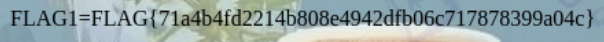
\includegraphics{flag3.png}

Jeszcze nie wyświetlała mi się cała za pierwszym razem, więc powiększyłem rozmiar iframe, ale to już taki szczegulik.

Kod ostatecznego footera w footer\_iframe.html.

\end{document}
